\documentclass[12pt,fleqn]{article}\usepackage{../../common}
\begin{document}
Eğrilik (Curvature)

Bir eğrimiz var, bu eğriye herhangi bir noktada ona en iyi uyan, onun eğimini en
iyi gösteren bir çemberi nasıl buluruz? Alttaki gibi bir uyumdan bahsediyoruz,

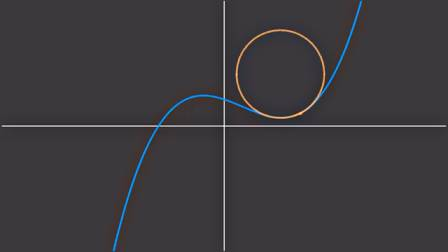
\includegraphics[width=15em]{calc_multi_60_01.jpg}

Bu yazıda bu ideal çemberin yarıçapını bulmayı göreceğiz, elde edilecek
formül eğrinin o noktadaki türevleri üzerinden yapılacak.

Çemberin bir $x_0,y_0$ merkezli olduğunu düşünelim, ve yarıçapı $r$ olsun. Bu
çemberin formülü şekildeki gibi olur,

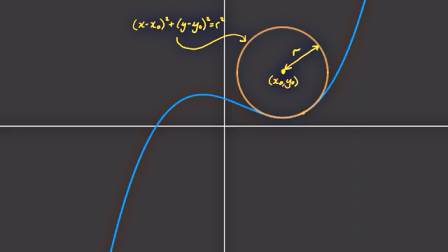
\includegraphics[width=15em]{calc_multi_60_02.jpg}

Şimdi cebirsel numaralara gelelim. Çember 

$$
(x-x_0)^2 + (y-y_0)^2 = r^2
$$

formülünün $x$'e göre türevini alalım. Karedeki 2 aşağı iner, ve parantez içinin
türevi alınır,

$$
2 (x-x_0) [1] + 2(y-y_0) \frac{\ud y}{\ud x} = 0
$$

$$
(x-x_0) + (y-y_0) \frac{\ud y}{\ud x} = 0
$$

Şimdi üstteki formülün bir kez daha türevini alalım,

$$
1 + (y-y_0) \frac{\ud^2y}{\ud x^2} +
\left(  \frac{\ud y}{\ud x}  \right) \frac{\ud y}{\ud x}  = 0
$$

$$
1 + (y-y_0) \frac{\ud^2y}{\ud x^2} +
\left(  \frac{\ud y}{\ud x}  \right)^2 = 0
$$

Böylece çember formülünden başlayarak üç tane formül elde etmiş olduk.

$$
(x-x_0)^2 + (y-y_0)^2 = r^2
\mlabel{1}
$$

$$
(x-x_0) + (y-y_0) \frac{\ud y}{\ud x} = 0
\mlabel{2}
$$

$$
1 + (y-y_0) \frac{\ud^2y}{\ud x^2} +
\left( \frac{\ud y}{\ud x}  \right)^2 = 0
\mlabel{3}
$$

(3) formülünü $y-y_0$ solda olacak şekilde tekrar düzenleyelim,

$$
y-y_0 = - \frac{1 + \left( \frac{\ud y}{\ud x}  \right)^2}{\frac{\ud^2y}{\ud x^2}}
$$

Benzer bir işlemi (2) üzerinde $x-x_0$ için yapalım,

$$
x-x_0 = -(y-y_0)\frac{\ud y}{\ud x}
$$

Üstteki formülde $y-y_0$ ifadesi var, onu iki üstteki formülde bulmuştuk,
oraya sokalım,

$$
= \frac{1 + \left( \frac{\ud y}{\ud x}  \right)^2}{\frac{\ud^2y}{\ud x^2}}
\frac{\ud y}{\ud x}
$$

Böylece hem $x-x_0$ hem de $y-y_0$ için bir formül elde etmiş olduk.

Bu formülleri cember formülü $r$ içine koyalım,

$$
\left[
    \frac{1 + \left( \frac{\ud y}{\ud x}  \right)^2}
         {\frac{\ud^2y}{\ud x^2}} \frac{\ud y}{\ud x}
\right]^2
+
\left[
  - \frac{1 + \left( \frac{\ud y}{\ud x}  \right)^2}
         {\frac{\ud^2y}{\ud x^2}}
\right] = r^2
$$

Ortak ifadeyi dışarı çekersek, 

$$
\left[
    \dfrac{1 + \left( \dfrac{\ud y}{\ud x}  \right)^2}
         {\dfrac{\ud^2y}{\ud x^2}}
\right]^2
\left(  \left(\dfrac{\ud y}{\ud x}  \right)^2 + 1 \right) = r^2
$$

$$
\frac{\left( 1 +  \left( \dfrac{\ud y}{\ud x} \right)^2  \right)^3}
     { \left( \dfrac{\ud^2y}{\ud x^2}   \right)^2  }
     = r^2
$$

Karekök alırsak,

$$
r =
\frac{\left( 1 +  \left( \dfrac{\ud y}{\ud x} \right)^2  \right)^{3/2}}
     { \dfrac{\ud^2y}{\ud x^2}   }
$$


Böylece sonuca erişmiş olduk. Çemberin türevlerini kullanarak o çemberin
yarıçapını formülize eden bir ifadeye eriştik. Eğrinin her noktada birer birinci
ve ikinci derece türevi vardır ve bu türevleri baz alarak oluşturulmuş bir
çember o noktada tabii ki o eğriyi en yakın yaklaşık olarak temsil eden
çember olacaktır. 

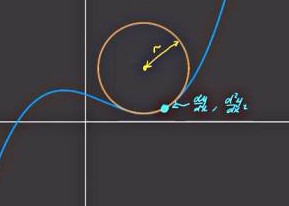
\includegraphics[width=10em]{calc_multi_60_03.jpg}
     
[devam edecek]

Kaynaklar

[1] Radius of Curvature Proof - approximating a curve with a circle!,
    \url{https://www.youtube.com/watch?v=ZCJfq77sFE8}

\end{document}
